\documentclass{report}
\usepackage[francais ]{babel}
\usepackage[utf8]{inputenc}
\usepackage[T1]{fontenc}
\usepackage{graphicx}
\usepackage{float}
\usepackage{hyperref}
\usepackage{array}
\title{\Huge Guide d'utilisateur \\ \huge Mini Games }

\author{M. \textsc{Friedli}, A. \textsc{Gillioz}, J. \textsc{Guerne}\\
He-Arc Ingénierie\\
2000 Neuchatel}
\date{\today{}}
\begin{document}
\maketitle

\chapter{Connexion}
Pour commencer à jouer il faut commencer par se connecter à un serveur.
Au lancement du programme vous devrez donc entrer l'adresse d'un serveur et aussi chsoir un pseudo. Une fois les champs remplis vous pouvez cliquer sur le bouton connecter pour tenter de vous connecter.

\begin{figure}[H]
	\centering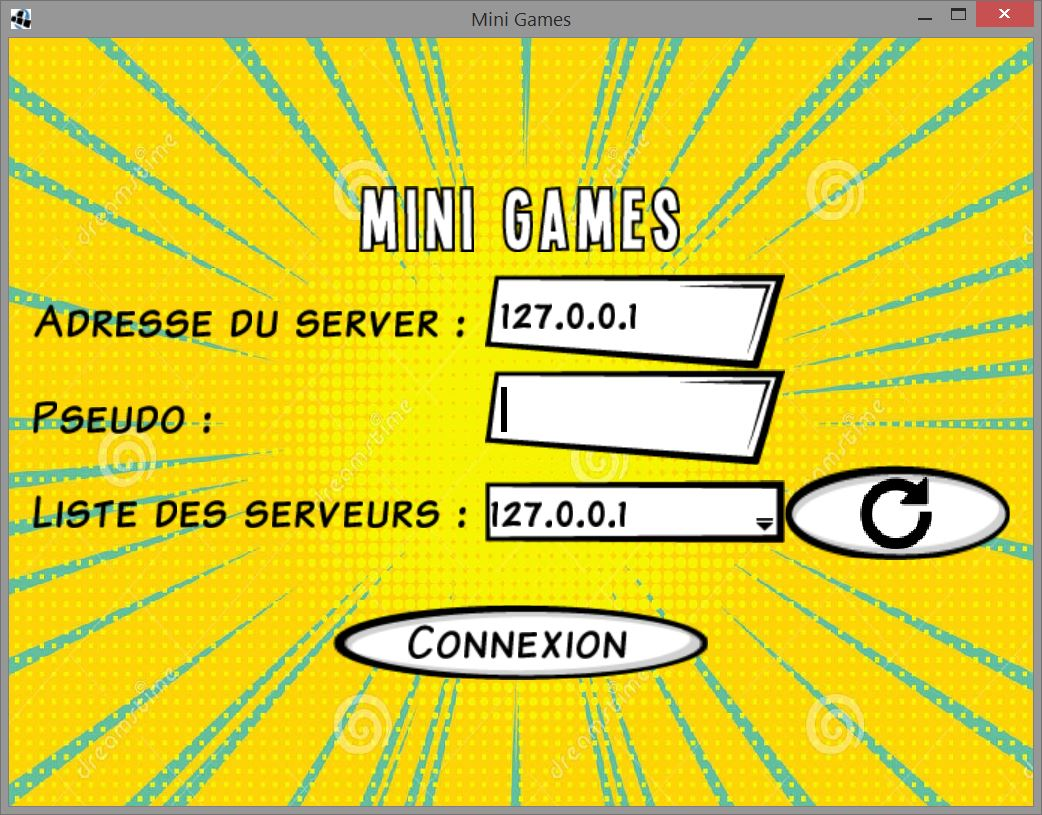
\includegraphics[width=9cm]{loginScreen}
	\caption{Écran de connexion}
\end{figure}

Pour faciliter la connexion au sevreur un système de recherche des serveurs est disponible. Le recherche se lance
automatiquement au démarrage du programme et peut être relancé à nouveau plus tards en appuyant sur le bouton de rafraichissament.


\chapter{Menu de sélection des minis jeux}
Une fois correctement connecté au serveur vous avez le choix de lancer une partie de morpion ou de bataille navale.
\begin{figure}[H]
	\centering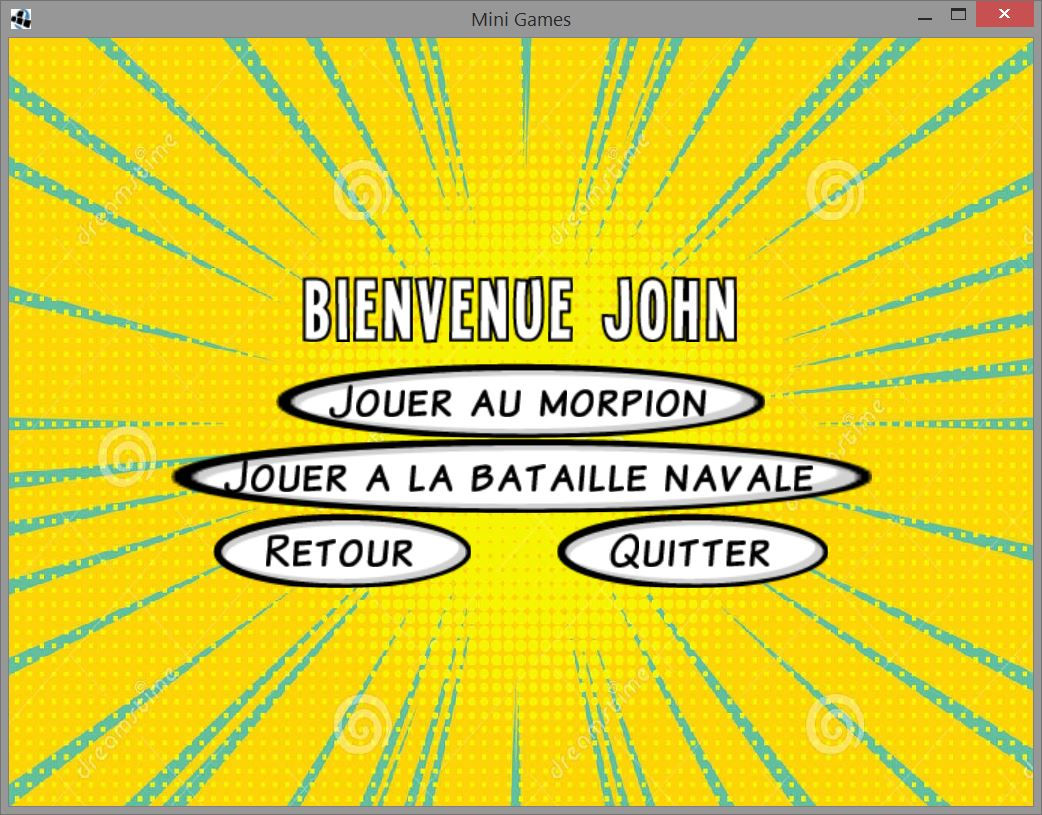
\includegraphics[width=9cm]{MenuJeux}
	\caption{Écran de connexion}
\end{figure}

Quand vous commencez une partie d'un jeu vous êtes dabord mis en attente puis
une fois un adversaire trouvé la partie commencera.

\begin{figure}[H]
	\centering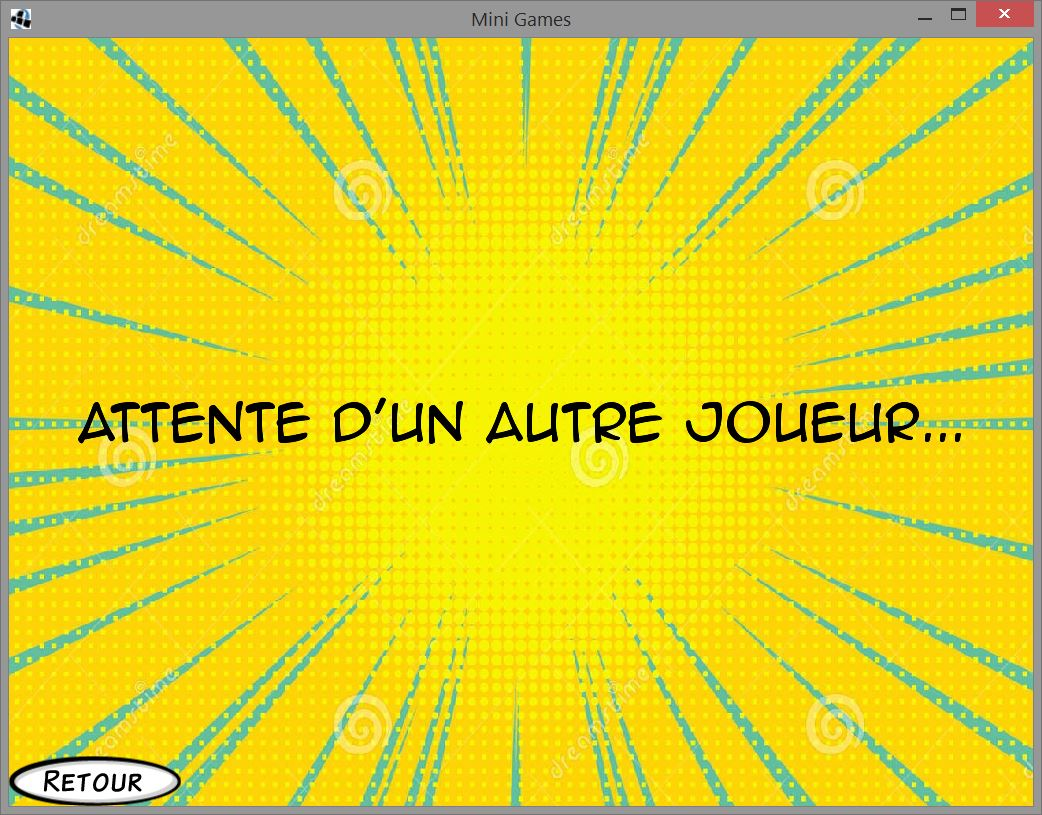
\includegraphics[width=9cm]{morpionwaiting}
	\caption{Écran d'attente}
\end{figure}

\chapter{Morpion}
Le morpion est un jeu qui se joue tour par tour où les joueurs vont placer sur un
plateau de jeu des caractères ('x' ou 'o'). Dès qu'une ligne ou une diagonale est remplie uniquement par un seul caractère
le joueur ayant rempli cette ligne/diagonale a gagné.

\begin{figure}[H]
	\centering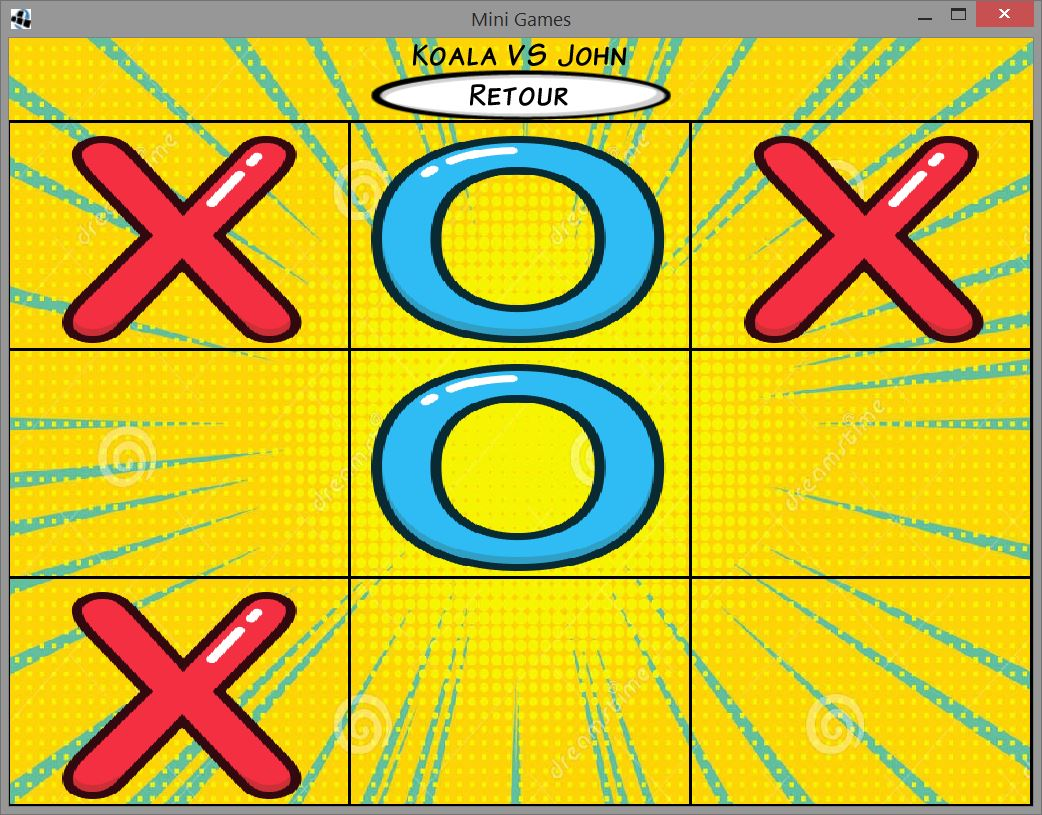
\includegraphics[width=9cm]{morpioningame}
	\caption{Écran de jeu du morpion}
\end{figure}


\chapter{Bataille navale}
Notre jeu de bataille navale, reprend les règles normales du jeu mais avec quelques différence sur le placement et la découverte des bateaux (ennemies ou aliés). Au lieu de pouvoir placer
des bateaux de taille variable, notre jeu permet de placer un bateau sur une seule et unique case
voir figure \ref{notreBataille}. Il s'agira alors pour notre adversaire de trouver nos bateaux sur la grille.

Au début de la partie le joueur doit placer ses bateaux sur le plateau de jeu une fois
tous les bateaux placés, le joueur peut cliquer sur le bouton "confirmer" pour valider le placment de ses bateaux.
Quand les deux adversaires ont fnis de placer leurs bateaux la partie peut commencer, le bouton "conirmer" change alors en un
bouton "inverser" permmettant à l'utilisateur d'afficher l'écran de ses bateaux ainsi que l'écran regroupant les endroits où il a tiré.


\end{document}
